\documentclass[12pt]{article}
\usepackage[utf8]{inputenc}

\usepackage{graphicx}
\graphicspath{ {images/} }

\usepackage[dvipsnames]{xcolor}

\usepackage{hyperref}
% \hypersetup{
    % colorlinks=true,
    % linkcolor=MidnightBlue,
    % citecolor=BrickRed,
    % urlcolor=BrickRed
% }

\title{
	{Code Generation for Event-B}\\
	{\large Innopolis University}\\
	{\large \textsc{Interim report}}\\
}

\author{Georgiy Krikun}
\date{5 December 2016}
% ---------------------------------------------------------------------------
\begin{document}

\setcounter{secnumdepth}{0}

\maketitle
\pagebreak
\begin{abstract}
  In this interim report I will describe specifics of my bachelor thesis work
  (which worth two courses).
  Actually I don't stop work on thesis, you could see latest version in 
  \href{https://github.com/kriku/thesis}{my repository}, and
  \href{https://kriku.github.io/thesis/paper/thesis.pdf}{the latest version}
  of this report as well.
\end{abstract}

\pagebreak
\tableofcontents

\pagebreak
\section{Goals of the project}
% Give a short summary of the main objectives of the project and the expected
% results. Provide an overview of the report, chapter by chapter.

The main objective of the project is implementation a translator from Event-B
modeling language to Eiffel programming language as Rodin platform plugin.

\href{http://poporo.uma.pt/EventB2Java/EventB2Java.html}
{Like it already be done} by Nestor Catano and Victor Rivera for translation from
Event-B to Java (or JML), before me.

But in my case I should implement plugin which translate Event-B model to Eiffel
Programming Language.\\

As results of work should be delivered working plugin, case study
(\href{http://poporo.uma.pt/EventB2Java/EventB2Java_studies.html}{or studies})
model in Event-B, translation of this model to Eiffel and proves of soundness of
the translator.\\

Overview of the report:\\
\begin{enumerate}
\item \textbf{Overview of System Specification}
  - section describes development specifics for Rodin Platform.
 
\item \textbf{Background Theory}
  - section describes formal approach, Event-B methodology, Eiffel
  Programming Language. 

\item \textbf{Overview of Task Specification and Project Schedule}
  - section consider plugin development decomposition to tasks, schedule
  timings and so on.

\item \textbf{Review of Tasks}
  - section describes current status of tasks.

\item \textbf{Interim Results}
  - section describes interim results of thesis work.

\item \textbf{Short Term Plans}
  - section states next steps I will take in project.

\end{enumerate}

\section{Overview of the System Specification}
% Provide an overview of the initial specification, setting out the main features
% of the system or project and addressing at least system functionality,
% interfaces (electronic and/or human), and signal/information representations. 

Whole system is a plugin for Rodin Platform. It uses translation rules
(\href{http://poporo.uma.pt/docs/rules.pdf}{like this one})
from Event-B to Eiffel and produce Eiffel code. Translation rules has been
provided to me by Victor Rivera. \\

\href{http://wiki.event-b.org/index.php/Plug-in_Tutorial}{Tutorial}
for the extension of the Rodin platform by plugin addition.

Access to plugin functionality will be granted through context menu of specific
machine, like in EventB2Java plugin:\\[2em]
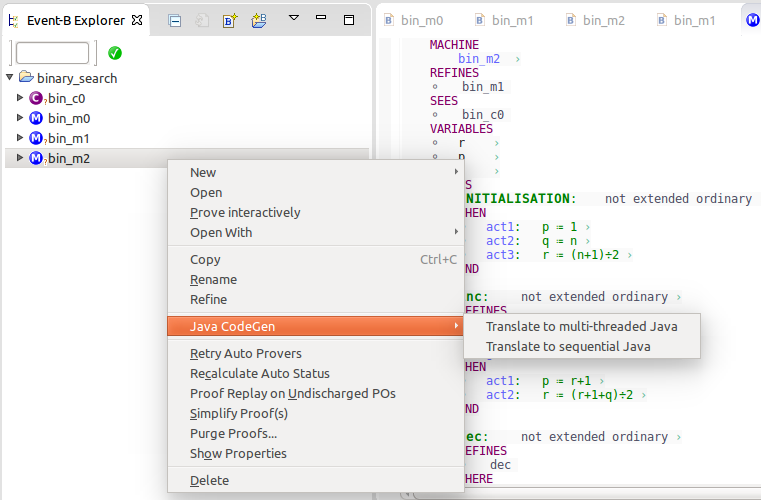
\includegraphics[width=\textwidth]{rodin_plugin}\\[2em]
But in my case it would be \texttt{Eiffel CodeGen} and will translate to Eiffel 
code.\\

\section{Background Theory}
% Describe the essential theory or theories to be applied in the thesis.

\subsection{Formal methods}
Formal methods are techniques used to model complex systems as
mathematical entities.

The primary idea behind a formal method is that there is benefit in writing a
precise specification of a system, and formal methods use a formal or
mathematical syntax to do so. This syntax is usually textual but can be
graphical. \\

Roughly speaking, formal design can be seen as a three step process:
\begin{enumerate}
\item \textbf{Formal Specification}
During the formal specification phase, the
engineer rigorously defines a system using a modeling language.
Modeling languages are fixed grammars which allow users to model
complex structures out of predefined types. This process of formal
specification is similar to the process of converting a word problem into
algebraic notation.

  \item \textbf{Verification}
As stated above, formal methods differ from other
specification systems by their heavy emphasis on provability and
correctness. By building a system using a formal specification, the
designer is actually developing a set of theorems about his system. 

  \item \textbf{Implementation}
Once the model has been specified and verified, it is implemented by converting
the specification into code. As the difference between software and hardware
design grows narrower, formal methods for developing embedded systems have been
developed. 

\end{enumerate}

\subsection{Event-B}

Event-B is another formal method for modelling complete developments of discrete
transition systems. Event-B was introduced by J-R. Abrial, and is derived from
the B method.

Unlike in B models, the static part of Event-B models is separated
from the dynamic part, and is referred to as ``contexts''. Thus, Event-B models
are composed of machines (the dynamic part. e.g. variables, invariants, events),
and contexts (the static part. e.g. carrier sets, constants).\\

Three basic relationships between machines and contexts are used to structure a
model:  

\begin{itemize}
  \item A machine \textbf{sees} a context
  \item A machine can \textbf{refine} another machine
  \item A context can \textbf{extend} another context
\end{itemize}

\begin{figure}[h]
  \centering
  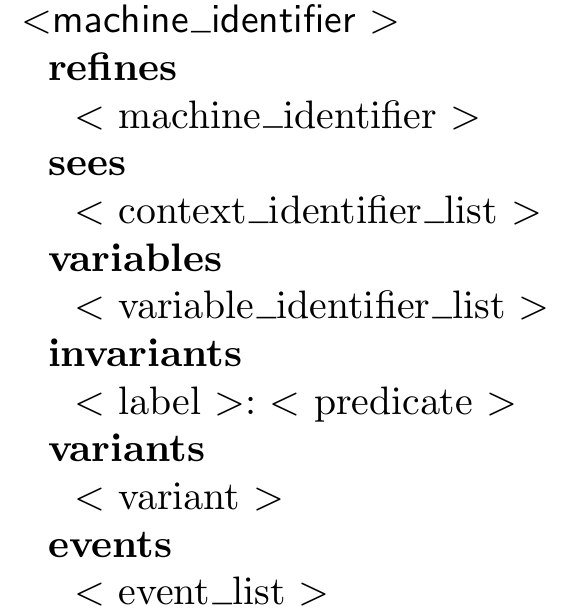
\includegraphics[width=0.4\linewidth]{event-b_machine}
  \caption{General structure of Event-B machine} 
\end{figure} 

\begin{figure}[h]
  \centering
  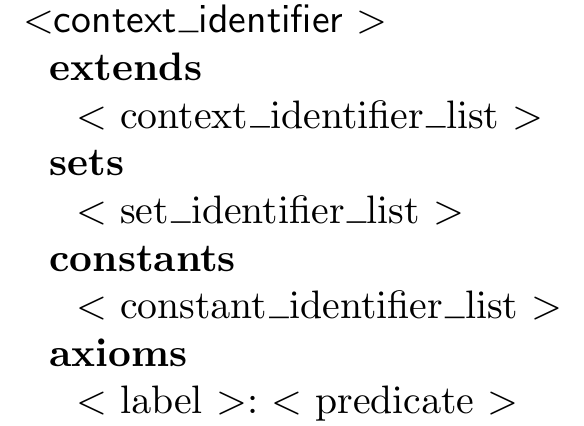
\includegraphics[width=0.4\linewidth]{event-b_context}
  \caption{General structure of Event-B context} 
\end{figure} 
This structure and method overall, well described by J-R. Abrial in \cite{eventb}

\subsection{Rodin Platform}

The
\href{http://wiki.event-b.org/index.php/Main_Page}{Rodin Platform}
is an Eclipse-based IDE for Event-B that provides effective
support for refinement and mathematical proof. The platform is open source,
contributes to the Eclipse framework and is further extendable with plugins.  


\section{Overview of Task Specification and Project Schedule}
List the primary tasks and sub-tasks required to carry out the project and an
overview of the project schedule, giving the timings (start date, duration,
amount of effort) of each task. List and discuss any changes that have been made
to the initial specification of the project. 
\section{Review of Tasks}

% Provide a comprehensive review of the status of each task and sub-task, setting out at
% least:
  % The status (not started, on-going, complete, behind schedule, ahead of
  % schedule ...); 
  % Problems encountered and identified solutions;
  % Anticipated problems and possible solutions;
  % Impact on the project schedule.

By now I slightly behind the schedule. Right now I think about case-study model
in Event-B and couldn't say that fully get ideas of the book.

As case-study I suggested modeling translator itself. It is interesting idea but
could be difficult and useless. As a plan 
 -- use existing translator to Java (EventB2Java) to get Java code and
tweak it to Rodin plugin. But Victor Rivera think it could be difficult for me,
and actually doing work twice. So right now I should decide whether I will model
translator itself (this will prove it soundness) or I will implement translation
rules in Java as plugin to Rodin, and then prove soundness of the translator.

So schedule depends on my decision and if I choose first way -- I do not have to
prove soundness (save about a month I think), but in any case I have to
implement ``the Visitor''.

All other task going right on schedule.
\section{Interim Results}
If possible, provide examples of any interim results you have achieved.
\section{Short Term Plans}
% Identify the next steps you will take in the project.

As next step -- I will implement ``Hello World'' plugin (just for get some
experience in plugin development). And finally decide whether I will do model of
translator in Event-B or not (by trying modeling, if I will fail it could be
the fate). 

\bibliographystyle{unsrt}
\bibliography{thesis}

\end{document}
